\documentclass[10pt, a4paper, oneside]{ctexbook}
\usepackage{amsmath, amsthm, amssymb, bm, graphicx, mathrsfs,esint}
\usepackage{hyperref}
\hypersetup{hypertex=true,
            colorlinks=true,
            linkcolor=blue,
            anchorcolor=blue,
            citecolor=blue}%用于公式引用
\title{{\Huge{\textbf{数学物理方法}}}\\Mathematical Methods in Physics}
\author{YLJ a.k.a. Natyiano}
\date{\today}
\linespread{1.5}
\newtheorem{theorem}{定理}[section]
\newtheorem{definition}[theorem]{定义}
\newtheorem{lemma}[theorem]{引理}
\newtheorem{corollary}[theorem]{推论}
\newtheorem{example}[theorem]{例}
\newtheorem{proposition}[theorem]{命题}
\newtheorem{method}[theorem]{方法}
\def\D{\mathrm{d}}
%\def\F{\ensuremath{f(z)}}
\def\Fex{\ensuremath{u(x,y)+iv(x,y)}}
\def\de{\ensuremath{\Delta}}
\newcommand{\partdev}[3][]
{\ensuremath{\frac{\displaystyle \partial^{#1} #2}{ \displaystyle \partial #3}}}
\newcommand{\F}[1][z]
{\ensuremath{f(#1)}}
\newcommand{\dev}[3][]
{\ensuremath{\frac{\displaystyle \D^{#1} #2}{ \displaystyle \D #3}}}
\begin{document}


\maketitle

\pagenumbering{roman}
\setcounter{page}{1}
\newpage
\pagenumbering{Roman}
\setcounter{page}{1}
\tableofcontents
\newpage
\setcounter{page}{1}
\pagenumbering{arabic}

\chapter{复数}
\textbf{约定}:
我们认为$z\in \mathbb{C}$,$x,y \in \mathbb{R}$
\section{定义以及运算}

\begin{definition}
    $$i=\sqrt{-1}$$
\end{definition}
称之为虚数单位。通过虚数单位和『实数单位($1$)』的线性组合,可以得到任意复数的表示方式:
$$z=x+iy,\;z\in \mathbb{C}, x\&y \in \mathbb{R}$$
$x,y$分别称为实部和虚部,记为:
\begin{align*}
    x=\text{Re}\;z\\y=\text{Im}\;z
\end{align*}
\begin{definition}
    $$z^*=x-yi$$
\end{definition}
称为$z$的共轭复数。容易得到,
\begin{align*}
    &z\cdot z^*=x^2+y^2=|z|^2 \ge 0 \\
    &x=\text{Re}\;z=\frac{z+z^*}{2} \\
    &y=\text{Im}\;z=\frac{z-z^*}{2i}
\end{align*}
注意到复数的运算与实数的运算存在许许多多的不同之处,例如
\begin{example}
    $$\lim_{y\to0}\frac{1}{x+yi}\ne \frac{1}{x}$$
    \begin{align*}
    \lim_{y\to0}\frac{1}{x+yi}=\lim_{y\to0}\frac{x-yi}{x^2+y^2}\to\\ \text{\rm Re} \;z= \begin{cases}
        0,\;x=0\\\displaystyle \frac{1}{x},\; x\ne 0
    \end{cases}\text{\rm Im} \;z= -i\pi \delta(x)
    \end{align*}
\end{example}
\section{复数的几何表示}
引入复平面可以容易地表示复数的几何形式:即$z=x+yi$在$x$轴(实轴)上的投影为$x$,在$y$轴(虚轴)上的投影为$y$。
那么,对应向量的(主)辐角$\theta$ 以及模$\rho$便定义为:
\begin{definition}
    $$\theta=\text{\rm Arg } z;\;\;\rho=\sqrt{x^2+y^2}$$
\end{definition}
主辐角记为Arg $\displaystyle z \in[-\pi,\pi] =\arctan \frac{y}{x}$,辐角记为arg $z$
那么得到:
\begin{lemma}
    \label{eularq}
    $$
    z = \rho(\cos \theta + i \sin \theta)
    $$
\end{lemma}
注意到:
$$
\frac{1}{z}=\frac{1}{\rho(\cos \theta + i \sin \theta)}=\frac{1}{\rho}(\cos \theta - i \sin \theta)
$$
\begin{lemma}
    \label{le1}
    假设$1/z=n\in \mathbb{C}$,
    $$\rho_{n}=1/\rho_z;\;\; {\rm arg \;} z=-{\rm arg \;} n$$
\end{lemma}
同样
\begin{lemma}
    \label{le2}
    假设$$
    z=\prod_{i=1}^{n}z_i\to \rho_z=\prod_{i=1}^n \rho_{z_i};\quad \text{\rm arg }z=\sum_{i=1}^n \text{\rm arg }z_i
    $$
    $$z_i\in\mathbb{C}$$
\end{lemma}
\begin{theorem}
    de Moivre’s 定理:
    $$z_1=\rho_1(\cos\theta_1+i\sin \theta_1)\quad z_2=\rho_2(\cos\theta_2+i\sin \theta_2)$$
    $$\Rightarrow$$
    $$z_1\cdot z_2=\rho_1\rho_2(\cos(\theta_1+\theta_2)+i\sin(\theta_1+\theta_2))$$
\end{theorem}
结合\ref{le1}和\ref{le2},我们可以得到任意个复数的乘法除法公式:
\begin{corollary}
    \begin{align*}
        z=\frac{\displaystyle\prod_{i=1}^n a_i \in \mathbb{C} }{\displaystyle\prod_{i=1}^n b_i \in \mathbb{C}}
        :\Longrightarrow \rho_z=\frac{\displaystyle\prod_{i=1}^n \rho_{a_i}}{\displaystyle\prod_{i=1}^n \rho_{b_i}} \quad \text{\rm arg }z = 
        \sum_{i=1}^n \text{\rm arg }a_i - \sum_{i=1}^n \text{\rm arg }b_i
    \end{align*}
\end{corollary}
\section{复数数列}
形式如下的序列称为复数数列
$$
z_n=x_n+i y_n , \; \; n=1,2,3,4,\dots
$$
$$z_n\text{ 收敛} \Leftrightarrow x_{n},y_{n} \text{ 收敛} $$
\section{欧拉公式以及复数的指数函数形式}

\begin{theorem}
    欧拉公式:
    $$e^{i\theta}=\cos \theta + i \sin \theta$$
\end{theorem}
\begin{proof}
    由 Taylor-Sereis
$$
e^x= \sum_{n=0}^\infty \frac{x^n}{n!}
$$
得到
$$
e^{i\theta}= \sum_{n=0}^\infty \frac{i^n\theta^n}{n!}=\left[ 1-\frac{\theta^2}{2}+\frac{\theta^4}{4!}+\dots \right]+ i \left[ \theta-\frac{\theta^3}{3!}+\dots \right]
$$
考虑到$\cos \theta$和$\sin \theta$ 的 Taylor-Series,得到:
$$
e^{i\theta}= \cos \theta + i \sin \theta
$$
\end{proof}
显然如上的证明并不是一个严格的证明,因为我们没有证明如上的展开适用于复数域,以及在交换次序时没有事先证明它绝对收敛。
结合\ref{eularq}得到$$z=\rho e^{i\theta}$$称为复数的指数函数形式。
\begin{example}
    计算无穷级数:$\cos \theta + \cos 2\theta + \cos 3\theta + \dots$
\end{example}
\begin{proof}
    原式等价于
    \begin{align*}
        \mathrm{Re} \;\; [e^{i\theta}+e^{i2\theta}+e^{i3\theta}+\dots]
    \end{align*}
    \begin{align*}
        e^{i\theta}+e^{i2\theta}+e^{i3\theta}+\dots\\
        =\lim_{n\to \infty} \frac{\displaystyle e^{i\theta}-e^{i(n+1)\theta}}{\displaystyle 1-e^{i\theta}}
    \end{align*}
\end{proof}

\section{复数域上的指数函数的反函数}
对于$\forall \; z\in \mathbb{C}$, 如何定义函数$g=f(z)=e^{z}$ 的反函数?
即定义一个函数,使得:
\begin{equation*}
    f^{-1}(g)=z
\end{equation*}
这个函数称为复对数函数,区别于$\mathbb{R}$上的指数函数$\ln(x)$。
\begin{definition}
    复对数函数:$$\mathrm{Ln}\;z=\ln |z| + i\mathrm{arg} \;z +2n\pi i$$
    $$s.t. \mathrm{Ln}\;g  = \mathrm{Ln}\; |z|e^{i\mathrm{arg}\;z+2ni\pi} $$
\end{definition}
其多值性来源于
$$
g=e^z=e^{z+2ni\pi}
$$

\chapter{复变序列}
对于某一复数序列$u_n=x_n+iy_n$,其和前$n$项和$S_n$:
\begin{equation*}
    \begin{aligned}
    &\sum_{n=0}^{\infty}\left(x_{n}+i y_{n}\right) \\
    &S_{n}=X_{n}+i Y_{n} \\
    &X_{n}=\sum_{i=0}^{n} x_{i}, Y_{n}=\sum_{j=0}^{n} y_{j}
    \end{aligned}
\end{equation*}
无穷级数收敛的充要条件:
$\forall\; \varepsilon > 0,\;\; \exists\; n>0;\;\; n \in \mathbb{Z}, \; s.t.\;\; \forall \; p>0\:$
\begin{equation*}
    \left|u_{n+1}+u_{n+2}+\ldots+u_{n+p}\right|<\varepsilon
\end{equation*}
级数收敛的必要条件:
\begin{equation*}
    \text{\boldmath Preliminary Test: } \lim_{n\to \infty} u_n = 0
\end{equation*}
\section{级数收敛性判别法}
\textbf{Test for alternating series}: An alternating series converges if the absolute value of the terms decreases steadily to zero, that is, if $\color{red} \left|a_{n+1}\right| \leq\left|a_{n}\right|$ and $\color{blue} \lim _{n \rightarrow \infty} a_{n}=0$.
\textbf{\color{red} 一致递减 \color{blue}至0}

\textbf{Comparison Method: }If $\exists N \in \mathbb{N}, \forall n>N$, the condition $\left|u_{n}\right|<v_{n}$ is satisfied. If $\displaystyle \sum_{n=0}^{\infty} v_{n}$ are convergent, then $\displaystyle \sum_{n=0}^{\infty}\left|u_{n}\right|$ are convergent.

\textbf{Ratio Method: }If there exists a constant $\rho$ ({\color{red} un-correlated with $n$ }), and $\left|u_{n+1} / u_{n}\right|<\rho<1$, then $\displaystyle \sum_{n=0}^{\infty} u_{n}$ are absolutely convergent.

\textbf{d'Alembert Method(Criterion): }级数的通项比值$\left(\displaystyle \frac{u_{n+1}}{u_n}\right)$的{\color{red}模}的上极限小于$1$,则原级数绝对收敛;级数的通项比值的模下极限大于1,则原级数发散。

\textbf{Gauss Method: }Assume that the ratio between two neighboring terms has the following form: $\displaystyle \frac{u_{n}}{u_{n+1}}=1+\frac{\mu}{n}+O\left(n^{-\lambda}\right)$
where $\mu=a+i b, \lambda>1$. 

If $a>1$, $\displaystyle \sum_{n=0}^{\infty} u_{n}$ absolutely convergent. 

If $\displaystyle a \leq 1, \sum_{n=0}^{\infty}\left|u_{n}\right|$ divergent.

\begin{example}
    使用 {\rm Gauss Method} 判别 级数$\displaystyle S_n=\sum_{n=0}^\infty \frac{1}{n}$的收敛性:
    \begin{align*}
        \frac{u_n}{u_{n+1}}=\frac{n+1}{n}=1+\frac{1}{n}
    \end{align*}
    则$a=1$,原级数发散。
    \newline
    使用 {\rm Gauss Method} 判别 级数$\displaystyle S_n=\sum_{n=0}^\infty \frac{1}{n^2}$的收敛性:
    \begin{align*}
        \frac{u_n}{u_{n+1}}=\left(\frac{n+1}{n}\right)^2=1+\frac{1}{n^2}+\frac{2}{n}
    \end{align*}
    则$a=2$,原级数绝对收敛。
\end{example}

\textbf{Cauchy Method: }$\displaystyle |u_n|^{1/n}$的上极限小于$1$,原级数绝对收敛;大于$1$,原级数发散。

\section{复数序列的一致收敛}

如果$S_n$一致收敛,则:
\begin{itemize}
    \item Continuity $u_{k}(z)$ is continuous in $G$, and $\sum_{k=1}^{\infty} u_{k}(z)$ is uniformly convergent, then $S(z)=\sum_{k=1}^{\infty} u_{k}(z)$ is continuous in $G$
    \item $\displaystyle
    \int_{C} \sum_{k=1}^{\infty} u_{k}(z) d z=\sum_{k=1}^{\infty} \int_{C} u_{k}(z) d z
    $
    \item $\displaystyle
        f(z)=\sum_{k=1}^{\infty} u_{k}(z) \text { is analytic in } G \to
        f^{(p)}(z)=\sum_{k=1}^{\infty} u_{k}^{(p)}(z)
        $
\end{itemize}

\section{幂级数与阿贝尔定理}

对于幂级数
\begin{equation*}
    \sum_{n=0}^{\infty} c_{n}(z-a)^{n}=c_{0}+c_{1}(z-a)+c_{2}(z-a)^{2}+\ldots
\end{equation*} 有
\begin{theorem}\rm
    \textbf{Abel theorem}: If the series $\displaystyle \sum_{n=0}^{\infty} c_{n}(z-a)^{n}$ are convergent at $z=z_{0}$, then
the series are absolutely convergent in a disk region (with a radius of $\left|z_{0}-a\right|$ ) surrounding $z_{0}$, and are uniformly convergent in the region $|z-a| \leq r\left(r<\left|z_{0}-a\right|\right)$.
\end{theorem}
\begin{corollary}\rm
    If $\displaystyle \sum_{n=0}^{\infty} c_{n}(z-a)^{n}$ are divergent at $z_{1}$, then also divergent in $|z-a|>\left|z_{1}-a\right|$.
\end{corollary}

\begin{figure}[h]
    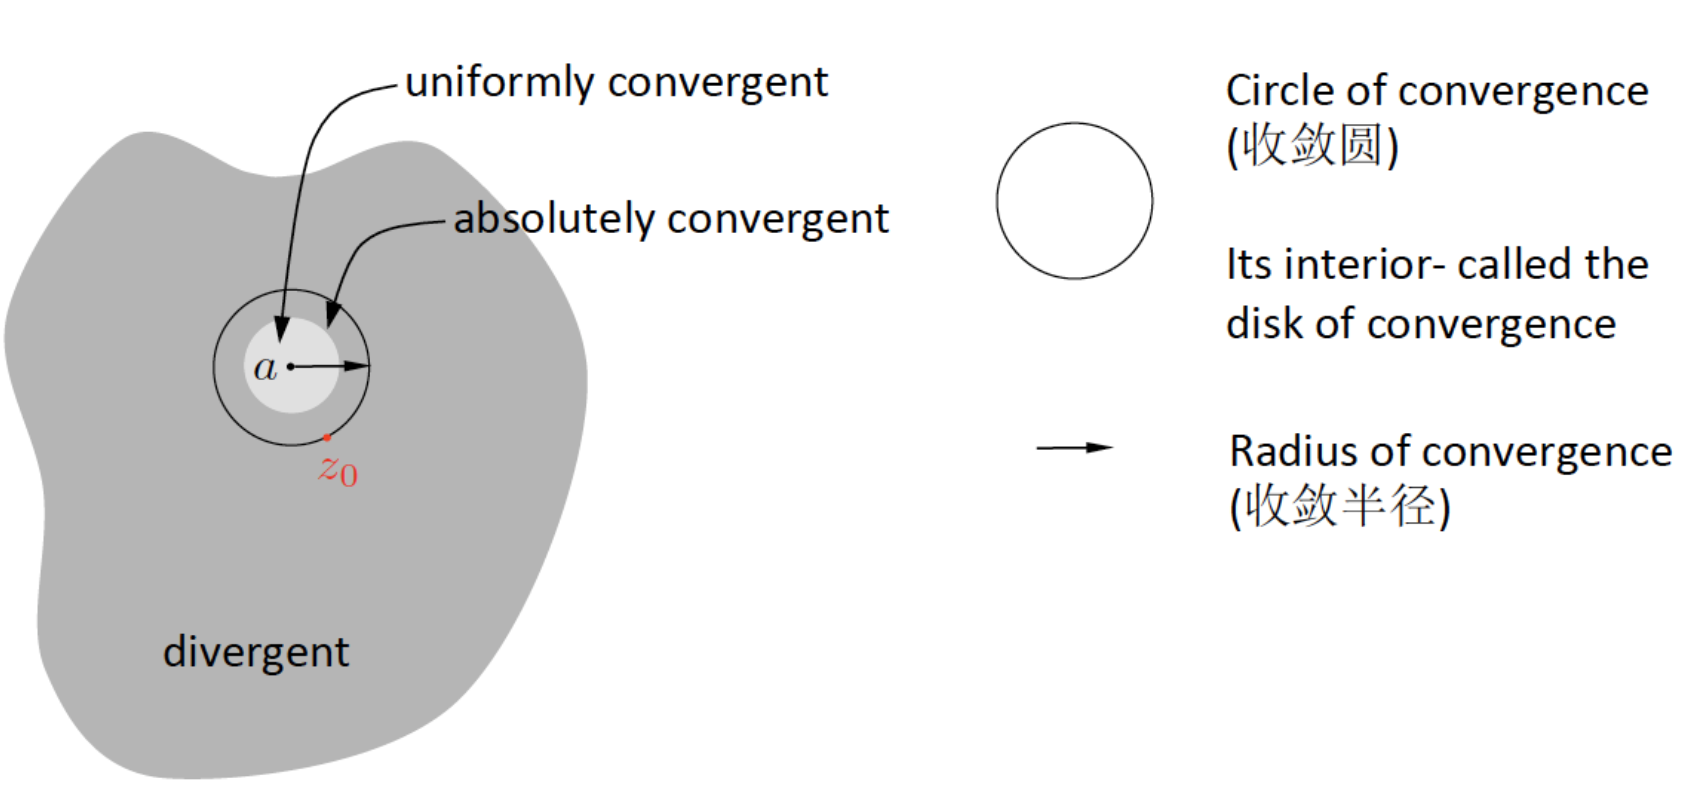
\includegraphics[width=0.9\textwidth]{./assets/converge_radius.png}
\end{figure}
\begin{method}
    {\rm \textbf{Cauchy-Hadamard Formula: }}
    \begin{equation*}
        R=\frac{1}{\overline{\lim }_{n \rightarrow \infty}\left|c_{n}\right|^{1 / n}}=\underline{\lim }_{n \rightarrow \infty}\left|\frac{1}{c_{n}}\right|^{1 / n}
    \end{equation*}
\end{method}
\begin{method}
    {\rm \textbf{d'Alembert Critrion: }}
    \begin{equation*}
        R=\lim _{n \rightarrow \infty}\left|\frac{c_{n}}{c_{n+1}}\right|
    \end{equation*}
\end{method}

\chapter{复变函数}
\section{复变函数的概念}
\begin{definition}
    复变函数是复数区域到复数区域的映射。
    $$f:\mathbb{C}\to \mathbb{C}$$
    $$f(z)=u(x,y)+iv(x,y)\quad z=x+iy\quad x,y\in \mathbb{R}$$
\end{definition}
与实变函数不同,{\color{red}区域}与{\color{red}区间}是有显著差异的。
\begin{definition}
    如果复平面上的点集$D$ 满足以下条件:
    \begin{enumerate}
        \item 开集性:不包含边界。 $\forall \; z_0 \in D ,\quad \exists \; \epsilon >0 \quad s.t. \; \left\{ z\;\mid\;|z-z_0|<\epsilon \right\} \subset D $
        \item 连通性:任意两点之间可以用区域内的线连通。
    \end{enumerate}
    那么点集$D$称为(开)区域。
    闭区域$$\overline{D}=D+\partial D$$
    $\partial D$是$D$区域的边界。边界具有方向,其正方向定义为使得区域位于运动方向的左手侧的方向。
\end{definition}
\begin{definition}
    双曲函数定义为:
$$
\begin{array}{lll}
\sinh (z)=\displaystyle\frac{e^{z}-e^{-z}}{2} & \cosh (z)=\displaystyle\frac{e^{z}+e^{-z}}{2} & \tanh (z)=\displaystyle\frac{\sinh (z)}{\cosh (z)} \\
\operatorname{coth}(z)=\displaystyle \frac{\cosh (z)}{\sinh (z)} & \operatorname{sech}(z)=\displaystyle \frac{1}{\cosh (z)} & \operatorname{csch}(z)=\displaystyle \frac{1}{\sinh (z)}
\end{array}
$$
\end{definition}
类比$\cos z, \sin z$可以得到:
双曲函数的周期性:
$$
\sinh (z) = \sinh (z+i2n\pi) \quad \cosh (z) = \cosh (z+i2n\pi) \quad \tanh(z)=\tanh(z+in\pi)\quad n\in\mathbb{Z}
$$
\begin{definition}
    函数$f^{-1}(z)$称为函数$f(z)$的逆函数,如果:
    $$
    f^{-1}(f(z))=z
    $$
\end{definition}

\section{单值性与黎曼面}
注意函数的多值性:
\begin{figure}[h]
    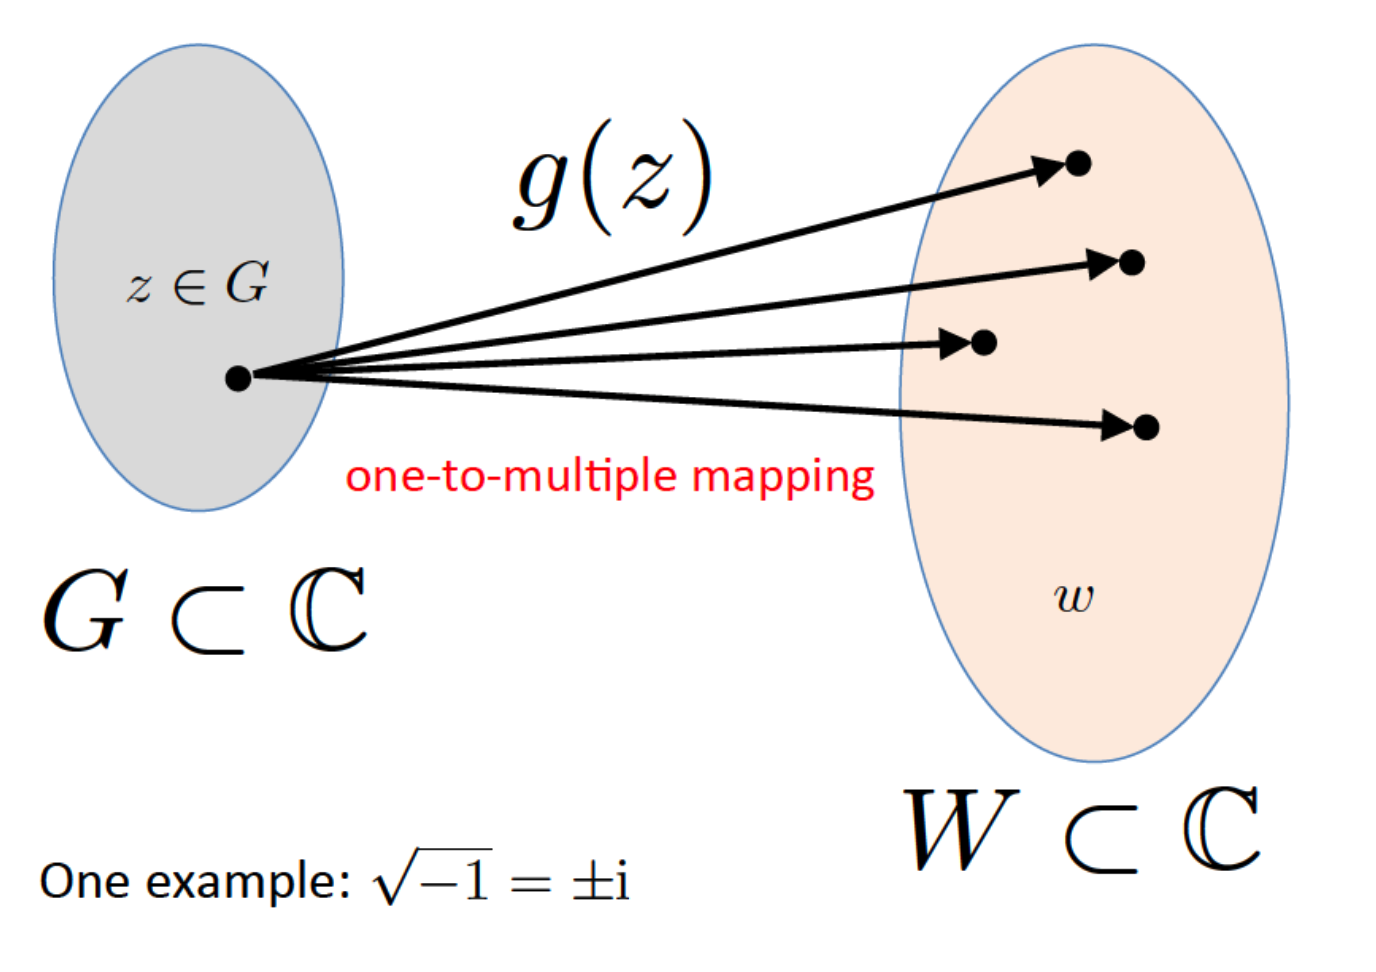
\includegraphics[width=0.9\textwidth]{./assets/multi-value.png}
\end{figure}
\begin{equation*}
    \text{定义域$G$}\quad z=x+i y \quad \xrightarrow{f(z)} \quad \text{值域$W$} \quad w=f(z)=u(x, y)+i v(x, y)
\end{equation*}
\begin{example}
    根式函数:$w=\sqrt[n]{z-a}$。令$z-a=re^{i\theta}$
    得到$w$有$n$个根:
    $$
    w_1=\sqrt[n]{r}e^{\theta/n}\quad
    w_2=\sqrt[n]{r}e^{\theta/n+2\pi/n}\quad
    \dots \quad
    w_n=\sqrt[n]{r}e^{\theta/n+2(n-1)\pi/n}
    $$
    辐角的多值性                                                           
\end{example}
\begin{example}
    对数函数:
$$
w=\ln z=\ln |z| +\textcolor{red}{i(\theta \pm 2n\pi)}
$$
\textcolor{red}{模的多值性}
\end{example}
反三角函数:
\begin{align*}
&\arcsin (z)=\frac{1}{i} \ln \left(i z+\sqrt{1-z^{2}}\right) \\ 
&\arccos (z)=\frac{1}{i} \ln \left(z+\sqrt{z^{2}-1}\right)\\ 
&\arctan (z)=\frac{1}{2 i} \ln \frac{1+i z}{1-i z}
\end{align*}
\begin{example}
    以$\arcsin z$为例:
    $$
\sin (w)=\frac{e^{i w}-e^{-i w}}{2 i}=z
$$
{\rm Multiply $e^{i w}$ for both sides, we have}
$$
\begin{aligned}
&\left(e^{i w}\right)^{2}-2 i z\left(e^{i w}\right)-1=0 \\
&e^{i w}=\frac{2 i z \pm \sqrt{4-4 z^{2}}}{2}=i z+\sqrt{1-z^{2}} \\
&\Rightarrow w=\frac{1}{i} \ln \left(i z+\sqrt{1-z^{2}}\right)
\end{aligned}
$$
\end{example}
复合函数多值性的判断:
\begin{example}
    $\sin \sqrt{z}$是多值函数(两个值),而$\cos \sqrt{z}$是单值函数。
\end{example}
\begin{definition}
    当自变量$z$围绕某点$z_0$旋转一圈(辐角增加$2\pi$)之后,若得到的新的函数与原函数不相等,则$z_0$称为一个支点。
\end{definition}
例如:
\begin{example}
    $w=\sqrt{z}$:
    $$z^\prime=z\cdot e^{2\pi i}\to w^\prime=\sqrt{z}\cdot e^{ \pi i} = - \sqrt{z} \ne w$$
    所以$z_1 = 0,\;z_2=\infty$是$w$的两个支点。
\end{example}

\begin{method}
    多值函数的单值化:
\begin{itemize}
    \item 限定辐角的范围,例如$(0,2\pi]$
    \item 规定某点$z_0$的值,然后描绘途径该点到目标点$z$的不同路径下的$f(z)$的取值。
\end{itemize}
\end{method}

\section{导数及解析函数的定义}
\begin{definition}
    $f(z)$在$z_0$以及其邻域上有定义,且沿任何路径$z\to z_0$
    时均有 $$\lim_{z\to z_0}f(z)=f(z_0)$$ 
    则$f(z)$在$z_0$上连续。
\end{definition}
\begin{definition}
    若$f(z)$在其定义域上处处连续,则称其为连续函数。
\end{definition}
\begin{definition}
    若$f(z)$在其$z_0$上连续,且沿任何路径$\Delta z \to 0$
    $$
    f' (z) =\lim_{\Delta z \to 0} \frac{f(z_0+\Delta z)-f(z_0)}{\Delta z}
    $$
    存在且唯一,则称$f(z)$在$z_0$可导。
\end{definition}
\begin{definition}
    若$f(z)$在$z_0$及其邻域各点均可导,则称为在$z_0$解析。
\end{definition}
\begin{definition}
    若$f(z)$在域$D$上处处解析,则称为$D$上的解析函数。
\end{definition}
\section{柯西-黎曼条件}
若$f(z)=u(x,y)+iv(x,y)$其中$u,v$均为二元实函数,
那么$f(z)$可导的必要条件之一为柯西-黎曼条件:
\begin{definition}{\rm Cauchy-Riemann Condition}:
    $$
    \left\{
    \begin{aligned}
        \frac{\displaystyle \partial u(x,y)}{ \displaystyle \partial x}=\frac{\displaystyle \partial v(x,y)}{\displaystyle \partial y}\\
        \frac{\displaystyle \partial v(x,y)}{ \displaystyle \partial x}=-\frac{\displaystyle \partial u(x,y)}{\displaystyle \partial y} 
    \end{aligned}     
    \right.
    $$
\end{definition}
极坐标的柯西黎曼条件:
\begin{align*}
    z=re^{i\theta}\Rightarrow \de z = \partdev{z}{r} \de r+ \partdev{z}{\theta} \de \theta =e^{i\theta}\de r + ire^{i\theta}\de \theta
\end{align*}
(1) Along $r$ direction $(\Delta \theta=0)$
\begin{equation*}
\lim _{\Delta r \rightarrow 0} \frac{\Delta u+i \Delta v}{\Delta r e^{i \theta}}=\frac{1}{e^{i \theta}}\left(\frac{\partial u}{\partial r}+i \frac{\partial v}{\partial r}\right)
\end{equation*}
(2) Along $\theta$ direction $(\Delta r=0)$
\begin{equation*}
\lim _{\Delta \theta \rightarrow 0} \frac{\Delta u+i \Delta v}{r \Delta \theta i \mathrm{e}^{i \theta}}=\frac{1}{r i e^{i \theta}}\left(\frac{\partial u}{\partial \theta}+i \frac{\partial v}{\partial \theta}\right)=\frac{1}{e^{i \theta}}\left(\frac{-i}{r} \frac{\partial u}{\partial \theta}+\frac{1}{r} \frac{\partial v}{\partial \theta}\right)
\end{equation*}
\begin{equation*}
    \Rightarrow \begin{cases} \displaystyle
        \partdev{u}{r}=\frac{1}{r} \partdev{v}{\theta}\\
       \displaystyle \partdev{v}{r}=-\frac{1}{r} \partdev{u}{\theta}
    \end{cases}
\end{equation*}
\begin{corollary}
    在某一个点,$f(z)$可导的充分必要条件:
    \begin{enumerate}
        \item 函数的实部和虚部均为二元可微实函数。
        \item 满足柯西黎曼条件。
    \end{enumerate}
\end{corollary}
\begin{proof}
    假设$f(z)=u(x,y)+iv(x,y)$,由条件1得:
    \begin{align*}
        \Delta u=\frac{\partial u}{\partial x}\Delta x+\frac{\partial u}{\partial y}\Delta y+\epsilon_1\Delta x+\epsilon_2 \Delta y \\
        \Delta v=\frac{\partial v}{\partial x}\Delta x+\frac{\partial v}{\partial y}\Delta y+\epsilon_3\Delta x+\epsilon_4 \Delta y \\
        \lim_{ \Delta x \to 0, \Delta y \to 0}  \epsilon_i =0 \quad i=1,2,3,4
    \end{align*}
    \begin{align*}
        \Delta f=\Delta u + i \Delta v=\frac{\partial u}{\partial x}\Delta x+\frac{\partial u}{\partial y}\Delta y+\epsilon_1\Delta x+\epsilon_2 \Delta y+\\
        i\left( \frac{\partial v}{\partial x}\Delta x+\frac{\partial v}{\partial y}\Delta y+\epsilon_3\Delta x+\epsilon_4 \Delta y \right)\\
        =\left(i\frac{\partial v}{\partial x}+\frac{\partial u}{\partial x}\right) \Delta x + \left(i\frac{\partial v}{\partial y}+\frac{\partial u}{\partial y}\right) \Delta y  +(\epsilon_1+i\epsilon_3)\Delta x +(\epsilon_2+i\epsilon_4)\Delta y\\
        =\left(i\frac{\partial v}{\partial x}+\frac{\partial u}{\partial x}\right) \Delta x + i\left(\frac{\partial v}{\partial y}-i\frac{\partial u}{\partial y}\right) \Delta y  +(\epsilon_1+i\epsilon_3)\Delta x +(\epsilon_2+i\epsilon_4)\Delta y\\
    \end{align*} 
    由条件2得:
    \begin{align*}
        \Delta f=\left(i\frac{\partial v}{\partial x}+\frac{\partial u}{\partial x}\right) \Delta z  +(\epsilon_1+i\epsilon_3)\Delta x +(\epsilon_2+i\epsilon_4)\Delta y\\
        z=x+iy\to\Delta z= \Delta x+i\Delta y\\
        \lim_{\Delta z \to 0} \frac{\Delta f}{\Delta z} = \frac{\partial u}{\partial x}+i\frac{\partial v}{\partial x}
    \end{align*}
\end{proof}
\begin{corollary}
    在某一个区域$G$内,$f(z)$解析的充分必要条件:
    \begin{enumerate}
        \item 函数的实部和虚部均为二元可微实函数,且其四个偏导$\left(\displaystyle \partdev{u}{x} \; \partdev{v}{x} \; \partdev{u}{y} \; \partdev{v}{y} \right)$连续。
        \item 满足柯西黎曼条件。
    \end{enumerate}
\end{corollary}
\textcolor{red}{注意:多值函数一定不可导,不解析。}
\begin{example}
    $e^z$在$z\to\infty$时一定不解析,因为其在$z\to\infty$时是多值的。同理,三角函数和双曲函数在$z\to\infty$时也是不可导的。
\end{example}


\section{解析函数的特性}
假设某个复变解析函数:$f(z)=u(x,y)+iv(x,y)\quad u,v\in \mathbb{R}$。由柯西-黎曼条件得到:
\begin{lemma}
    \begin{equation}
    \label{laplace}
        \frac{\displaystyle \partial^2 u(x,y)}{ \displaystyle \partial^2 x}+\frac{\displaystyle \partial^2 u(x,y)}{\displaystyle \partial^2 y}=0
    \end{equation}
    \begin{equation}
        \label{laplace2}
            \frac{\displaystyle \partial^2 v(x,y)}{ \displaystyle \partial^2 x}+\frac{\displaystyle \partial^2 v(x,y)}{\displaystyle \partial^2 y}=0
        \end{equation}
\end{lemma}
\ref{laplace}和\ref{laplace2} 是拉普拉斯方程。所以解析函数的实部和虚部均为调和函数。即:
\begin{equation*}
    \begin{aligned}
    &\Delta u=\nabla^{2} u=\frac{\partial^{2} u}{\partial x^{2}}+\frac{\partial^{2} u}{\partial y^{2}}=0 \\
    &\Delta v=\nabla^{2} v=\frac{\partial^{2} v}{\partial x^{2}}+\frac{\partial^{2} v}{\partial y^{2}}=0
    \end{aligned}
    \end{equation*}
\begin{theorem}
    $$\frac{\displaystyle \partial f(z)}{ \displaystyle \partial z^*}=0$$
    即解析函数与其自变量的共轭无关。
\end{theorem}
\begin{proof}
    $$x=\frac{z+z^*}{2},\quad y=\frac{z-z^*}{2}$$
    \begin{align*}
    \frac{\displaystyle \partial f(z)}{ \displaystyle \partial z^*}=\frac{\displaystyle \partial f(z)}{ \displaystyle \partial x}\frac{\displaystyle \partial x}{ \displaystyle \partial z^*}+\frac{\displaystyle \partial f(z)}{ \displaystyle \partial y}\frac{\displaystyle \partial y}{ \displaystyle \partial z^*}=\\
    \frac{1}{2}\left[\frac{\displaystyle \partial u}{ \displaystyle \partial x}-\frac{\displaystyle \partial v}{ \displaystyle \partial y}\right]+\frac{i}{2}\left[ \frac{\displaystyle \partial u}{ \displaystyle \partial y}+\frac{\displaystyle \partial v}{ \displaystyle \partial x} \right]=0
    \end{align*}
\end{proof}
\begin{theorem}
    解析函数的实部和虚部的等值线的切向量相互垂直。
\end{theorem}
\begin{proof}
    \begin{equation*}
        u(x, y)=C \Rightarrow \D u(x, y)=\frac{\partial u}{\partial x} \D x+\frac{\partial u}{\partial y} \D y=0
    \end{equation*}
    $\D \vec{s}$是实部等值线的切向量,则
    \begin{equation*}
        \D \vec{s}=(\D x, \D y) \propto\left(\frac{\partial u}{\partial y},-\frac{\partial u}{\partial x}\right)
    \end{equation*}
    \begin{equation*}
        v(x, y)=C^{\prime} \Rightarrow \D v(x,y)=\partdev{v}{x} \D x + \partdev{v}{y}\D y =0
    \end{equation*}
    $\D \vec{s'}$是虚部等值线的切向量,则
    \begin{equation*}
        \D \vec{s'} =\left(\D x^{\prime}, \D y^{\prime}\right) \propto\left(\frac{\partial v}{\partial y},-\frac{\partial v}{\partial x}\right)
    \end{equation*}
    \begin{equation*}
        \D \vec{s} \cdot \D \vec{s'} \propto\left(\frac{\partial u}{\partial y},-\frac{\partial u}{\partial x}\right) \cdot\left(\frac{\partial v}{\partial y},-\frac{\partial v}{\partial x}\right)=0 \Rightarrow \D \vec{s} \perp \D \vec{s'}
    \end{equation*}
\end{proof}
\section{由部分确定整个解析函数}
如果已知某个解析函数的实部$u(x,y)$以及在某点$z_0$的取值,可以确定整个解析函数:
\begin{method}
    由于柯西-黎曼条件,
$$\partdev{u(x,y)}{x}=\partdev{v(x,y)}{y}\to v(x,y)=\int \partdev{v}{x}\D x + h(y)$$
$$\partdev{u(x,y)}{y}=-\partdev{v(x,y)}{x}\to v(x,y)=-\int \partdev{u}{y}\D x + h(y)$$
$$\Rightarrow$$
$$\partdev{v(x,y)}{y}=-\int \partdev[2]{u}{y^2} \D x+h'(y)=\partdev{u(x,y)}{x}$$
$$\Rightarrow$$
$$h'(y)=\partdev{u(x,y)}{x}+\int \partdev[2]{u(x,y)}{y^2}\D x\to h(y)=\int h'(y)\D y + C$$
\end{method}
\begin{method}
    利用 C-R 条件,先找到解析函数的导数:
    $$\dev{f}{z}=\partdev{f}{x}=\partdev{u}{x}+i\partdev{v}{x}=\partdev{u}{x}-i\partdev{u}{y} \equiv g(z)$$
    $$\Rightarrow$$
    $$f(z)=\int g(z)\D z + C$$
\end{method}
\begin{method}
    $$f(z)=u(x,y)+iv(x,y),\quad f^*(z)=u(x,y)-iv(x,y)$$
    $$\Rightarrow$$
    $$u(x,y)=\frac{f(z)+f^*(z)}{2},\quad v(x,y)=\frac{f(z)-f^*(z)}{2i}$$
    通过代数运算,我们可以将$u(x,y)$写成:
    $$u(x,y)=u\left(\frac{z+z^*}{2},\frac{z-z^*}{2i}\right)=h(z)+h^*(z)=\left[h(z)+iC\right]+\left[h(z)+iC\right]^*$$
    对比系数可得:
    $$f(z)=2h(z)+2iC$$
\end{method}

\chapter{ 复变函数的积分}

\section{解析函数的积分特性}

\begin{definition}
    复变函数的积分定义为:
    $$\int_L f(z) \D z \equiv \lim_{n\to\infty}\sum_{j=1}^n f(\xi_j)(z_j-z_{j-1})$$
    其中$L$为有向路径。
\end{definition}
一些较为常用的性质:
$$\int_L f_1(z)+f_2(z)\D z=\int_L f_1(z)\D z+\int_L f_2(z)\D z$$
$$\int_L f(z)\D z = -\int_{-L} f(z)\D z$$
$$\int_{L_1+L_2} f(z)\D z = \int_{L_1} f(z)\D z+\int_{L_2} f(z)\D z$$
$$\int_{C} a f(z) d z=a \int_{C} f(z) d z \quad \text{where $a$ is a constant complex number}$$ 
\begin{equation*}
\left|\int_{C} f(z) d z\right| \leq \int_{C}|f(z)||d z|
\end{equation*}
$$\left|\int_{C} f(z) d z\right| \leq M l \quad \text{where $M$ is upper bound of $f(z)$}$$
\begin{theorem}
    单连通域上解析函数的柯西积分定理:假设$C$是某个单连通域的边界。
    $$\ointctrclockwise_C \F \D z = 0$$
\end{theorem}
\begin{proof}
    假设将复变解析函数$\F$沿着某一单连通域做回路积分:
\begin{equation}
    \label{int1}
    \ointctrclockwise_C \F \D z = \ointctrclockwise_C \left[\Fex\right](\D x + i \D y)
\end{equation}
其中正方向定义为确保解析区域在左手边的方向。展开\ref{int1}得到:
$$\ointctrclockwise_C \left[u\D x- v\D y\right] + i \ointctrclockwise_C \left[u\D y+ v\D x\right]$$
由格林公式
$$\ointctrclockwise_C \left[P\D x+ Q\D y\right] = \iint_\Sigma \left[-\partdev{P}{y}+\partdev{Q}{x}\right]\D x\D y$$
得到:
\begin{equation}
    \label{int2}
    \ointctrclockwise_C \F \D z=  \iint_\Sigma \left[-\partdev{u}{y}-\partdev{v}{x}\right]\D x\D y+i\iint_{\Sigma} \left[\partdev{u}{x}-\partdev{v}{y}\right]\D x\D y
\end{equation}
考虑{\rm C-R}条件,
$$\ref{int2}\equiv 0$$
\end{proof}
\begin{theorem}
    \label{cit2}
    复连通域上解析函数的柯西积分定理:
    假设$C$是一个复连通域的边界,而填上这个复连通域中的$C_1,C_2,\dots,C_N$所围成的区域可以将该域变为单连通域。那么:
    $$ \ointctrclockwise_C \F \D z= \sum_{n=1}^N \ointctrclockwise_{C_n} \F \D z$$
\end{theorem}
\begin{example}
Find the value of $\displaystyle \oint_{C} z^{n} d z$, where $n$ is an integer, $C$ is a simply closed curve in $\mathbb{C}$.
\begin{itemize} \rm
\item  If $n$ is non-negative, $z^{n}$ is analytic, then $\displaystyle \oint_{C} z^{n} d z=0$.
\item  If $n$ is negative, and if the contour does not enclose $z=0$, then $z^{n}$ is analytic inside the region bounded by $C$, and again we have $\displaystyle \oint_{C} z^{n} d z=0$.
\item  If $n$ is negative, and if the contour encloses $z=0$. We can draw a simple circle around $z=0$, and apply the Cauchy theorem for a multi-connected 
\end{itemize}
\begin{equation*}
\oint_{C} z^{n} d z=\oint_{|z|=\varepsilon} z^{n} d z=\int_{0}^{2 \pi} \varepsilon^{n+1} e^{\mathrm{i}(n+1) \theta} \mathrm{i} d \theta=\left\{\begin{array}{l}
2 \pi \mathrm{i}, n=-1 ; \\
0, n=-2,-3,-4, \ldots
\end{array}\right.
\end{equation*}
\end{example}
\begin{corollary}
    函数$f(z)$在$\Sigma_G$内解析,如果$\Sigma_C\subset \Sigma_G$,其线积分$\displaystyle \int_C f(z)\D z$ 与路径无关。
\end{corollary}
\section{柯西积分公式}
\begin{theorem}
    柯西积分公式:假设$C$包围了$\F$的单连通解析区域,$z_0$为区域内一点,则
    $$\F[z_0]=\frac{1}{2\pi i}\ointctrclockwise_C \frac{\F}{z-z_0}\D z$$
\end{theorem}
\begin{proof}
    不妨用一个小圆将$z_0$包围,其边界设为$\displaystyle C_r: \;\;\forall \; z\in \Sigma_{C_r}\quad z=z_0+re^{i\theta}$,则由\ref{cit2},
    \begin{align}
        \ointctrclockwise_C \frac{\F}{z-z_0}\D z=&\ointctrclockwise_{C_r}\frac{\F}{z-z_0}\D z= \notag\\
        \int_0^{2\pi}\frac{\F[z_0+re^{i\theta}]}{re^{i\theta}}ire^{i\theta}\D \theta=&
        i\int_{0}^{2\pi}\F[z_0+re^{i\theta}]\D \theta\label{cie}
    \end{align}
    再不妨令$r\to0$,那么\ref{cie}化为
    $$i\int_{0}^{2\pi}\F[z_0]\D \theta=2\pi i \F[z_0]$$
    即:
    \begin{equation}
    \label{prof}
    \ointctrclockwise_C \frac{\F}{z-z_0}\D z=2\pi i \F[z_0]
    \end{equation}
\end{proof}
\begin{lemma}
    令\ref{prof}中的$\F=1$,推出公式:
    \begin{align*}
        \frac{1}{2\pi i}\ointctrclockwise_C \frac{1}{z-z_0} \D z=
        \begin{cases}
            1\quad z_0\in \Sigma_C\\
            0\quad z_0\notin \Sigma_C
        \end{cases}
    \end{align*}
\end{lemma}
可以利用\ref{prof}计算解析函数的导数:
\begin{method}
    \label{method283}
    $$
    \F = \frac{1}{2\pi i}\ointctrclockwise_C \frac{\F[\xi]}{\xi-z}\D \xi \to
    $$
    $$
    f'(z)=\frac{1}{2\pi i} \dev{}{z}\ointctrclockwise_C \frac{\F[\xi]}{\xi - z}\D \xi= \frac{1}{2\pi i}\ointctrclockwise_C \frac{\F[\xi]}{(\xi-z)^2}\D \xi \to
    $$
    $$
    f''(z)=\frac{2!}{2\pi i}\ointctrclockwise_C \frac{\F[\xi]}{(\xi-z)^3}\D \xi 
    $$
    $$\dots$$
    $$
    f^{(n)}(z)=\frac{n!}{2\pi i}\ointctrclockwise_C \frac{\F[\xi]}{(\xi-z)^{n+1}}\D \xi
    $$
    这说明解析函数是任意阶可导的。
\end{method}
\section{最大模定理}
\begin{theorem}
    最大模定理:设$\F$在闭区域上解析,则其模$|\F|$的最大值只能出现在该区域的边界上,除非$\F$是一个常函数。
\end{theorem}
\begin{proof}
    \begin{align*}
        f^n(z)=\frac{1}{2\pi i} \ointctrclockwise \frac{f^n(\xi)}{\xi-z}\D \xi\\
        |\F|^n=|\left[\F\right]^n|=\left|\frac{1}{2\pi i} \ointctrclockwise \frac{f^n(\xi)}{\xi-z}\D \xi\right| \\ \le \frac{1}{2\pi} \ointctrclockwise \frac{|f(\xi)^n|}{|\xi-z|}|\D \xi|
        \le \frac{M^n}{2\pi d}\ointctrclockwise_C |\D \xi|=\frac{M^n}{2\pi d}l
    \end{align*}
    $d$为$z$至边界的最短距离,$\forall\; z:\;|z-\xi|\ge d$\\
    $M$为$|\F[\xi]|$的最大值,$\forall\; z:|f(\xi)|\le M,\;\xi\in C$\\
    即
    $$
    |\F|\le M\left[\frac{l}{2\pi d}\right]^{1/n}\to|\F|\le \lim_{n\to \infty} M\left[\frac{l}{2\pi d}\right]^{1/n}=M
    $$
    即
    $f(z),\;z\in \overline{\Sigma_C}$的最大值便是$f(\xi),\;\xi\in C$的最大值。
\end{proof}
\section{复变函数在其解析圆域上的泰勒级数展开}
    $\F$在$z_0$为圆心的圆域内解析,则对于任意一圆域内点$z$,有
    \begin{align*}
        f&(z)=\sum_{n=0}^\infty a_n(z-z_0)^n\\
        a&_n=\frac{1}{2\pi i}\ointctrclockwise \frac{\F[\xi]}{(\xi-z_0)^{n+1}}\D \xi=\frac{f^{(n)}(z_0)}{n!}
    \end{align*}
\begin{proof}
    \begin{align*}
        \F&=\frac{1}{2\pi i}\ointctrclockwise_C \frac{\F[\xi]}{\xi-z}\D \xi=\frac{1}{2\pi i}\ointctrclockwise_C \frac{\F[\xi]}{(\xi-z_0)-(z-z_0)}\D \xi\\
        &=\frac{1}{2\pi i}\ointctrclockwise_C \frac{\F[\xi]}{\xi-z_0}\frac{1}{1-\frac{z-z_0}{\xi-z_0}}\D \xi
    \end{align*}
    由于
    $$
    \frac{z-z_0}{\xi-z_0}\le 1,\quad\frac{1}{1-t}=\sum_{n=0}^\infty t^n,\;\; |t|<1
    $$
    \begin{align*}
    &\frac{1}{2\pi i}\ointctrclockwise_C \frac{\F[\xi]}{\xi-z_0}\frac{1}{1-\frac{z-z_0}{\xi-z_0}}\D \xi=\frac{1}{2\pi i}\ointctrclockwise_C \frac{\F[\xi]}{\xi-z_0}\sum_{n=0}^\infty \left[\frac{z-z_0}{\xi-z_0}\right]^n\D \xi=\\
    &\sum_{n=0}^\infty \left[\frac{1}{2\pi i}\ointctrclockwise_C \frac{\F[\xi]}{(\xi-z_0)^{n+1}}\D \xi\right](z-z_0)^n=\F
    \end{align*}
\end{proof}
复变函数在其解析圆域上的泰勒级数展开的收敛半径为:
$$
R=\lim_{n\to \infty}\frac{1}{\sqrt[n]{|a_n|}}=\lim_{n\to \infty} \left| \frac{a_n}{a_{n+1}} \right| \;\; or \;\; R=|z_0-z_1| \;\; \text{$z_1$是离$z_0$最近的奇点}
$$
\section{利用泰勒级数讨论最大模定理}
\begin{definition}
    Kronecker-$\delta$符号:
    \begin{equation}
        \delta_{mn}\equiv\frac{1}{2\pi}\int_0^{2\pi}e^i(n-m)\theta \D \theta=\begin{aligned}
            \notag
            \begin{cases}
                0,\quad m\ne n\\ 1,\quad m=n
            \end{cases}
        \end{aligned}
    \end{equation}
\end{definition}
假设最大模定理不成立,即:$$
\exists\;z_0\in\Sigma,\;z_0\notin \partial \Sigma\;\; s.t.\;|\F[z_0]|=\mathrm{max}\;|\F|
$$
那么以$z_0$为中心做泰勒展开:
$$
\F=\sum_{n=1}^\infty a_n (z-z_0)^n\to a_0=\F[z_0]
$$
由于
$$
z-z_0=re^{i\theta}
$$
\begin{align}
    |a_0|^2&=\frac{1}{2\pi} \int_{0}^{2\pi} |a_0|^2\D \theta=\frac{1}{2\pi}\int_0^{2\pi}|f(z_0)|^2 \D \theta\ge\frac{1}{2\pi}\int_0^{2\pi}f^*(z)\cdot f(z) \D \theta \notag\\ \notag
    &=\frac{1}{2\pi}\int_0^{2\pi}\sum_{m=1}^\infty a_m^* [(z-z_0)^*]^m\cdot \sum_{n=1}^\infty a_n (z-z_0)^n \D \theta\\\notag
    &=\sum_{m,n=0}^\infty a^*_m a_n r^{m+n}\frac{1}{2\pi} \int_0^{2\pi} e^{i(n-m)\theta}\D \theta \\\notag
    &=\sum_{m,n=0}^\infty a^*_m a_n r^{m+n}\delta_{mn}=\sum_{n=0}^\infty a^*_na_n r^{2n}=\sum_{n=0}^\infty |a_n|^2 r^{2n}\\
    &=|a_0|^2+\sum_{n=1}^\infty |a_n|^2r^{2n} \label{mmt1}
\end{align}
考虑到
$$
\sum_{n=1}^\infty |a_n|^2r^{2n}\ge 0 \Rightarrow |a_0|^2+\sum_{n=1}^\infty |a_n|^2r^{2n} \ge |a_0|^2
$$
若想要\ref{mmt1}成立,那么
$$
\sum_{n=1}^\infty |a_n|^2r^{2n} =0 \to a_n = 0 \to \F = constant.
$$
\begin{theorem}
    刘维尔定理:在全复平面内解析且有界的复变函数必为常函数。
\end{theorem}
\begin{proof}
    以$z_0=0$为中心做泰勒展开:
    $$
    \F = \sum_{n=0}^\infty a_n z^n,\quad a_n=\frac{1}{2\pi i}\ointctrclockwise_C \frac{\F[\xi]}{\xi^{n+1}}\D \xi
    $$
    由于$$
    \xi \in C\to \xi = re^{i\theta}\to \D \xi = ire^{i\theta} \D \theta
    $$
    则$|a_n|$可以化为
    $$
    |a_n|\le \frac{1}{2\pi}\ointctrclockwise_C \frac{|\F[\xi]|}{|\xi^{n+1}|}|\D \xi| \le \frac{1}{2\pi}\int_0^{2\pi} \frac{M}{r^{n}}\D \theta = \frac{M}{r^n}
    $$
    由于$\F$在整个复平面上解析,即其泰勒展开的收敛半径$R=\infty$,那么
    $$
    |a_n|\le \lim_{r\to \infty} \frac{M}{r^n} = 0 \to  \forall n\ne 0:\;a_n=0\;
    $$
\end{proof}
\section{解析函数的零点及其孤立性}
\begin{definition}
    $\F$在$z_0$点有$f(z_0)=0$,且在以$z_0$为圆心的圆域内的泰勒级数展开式最低幂次(最小的使得$a_n\ne0$的$n$)为$k$次,则称$z_0$为$\F$的$k-$阶零点。
\end{definition}
由定义得到,若$z_0$是$\F$的$k$-阶零点,则
$\forall\;k>n>0: \; f^{(n)}(z_0)=0$
\begin{theorem}
    零点的孤立性:假设$z_0$为$\F$的一个零点,则
    $$
    \exists\; r > 0 \; s.t. \; \forall z \in \{z \mid |z-z_0|<r\},\; f(z) \ne 0
    $$
    即零点不能构成区域。
\end{theorem}
\begin{proof}
    假设$z_0$为$\F$的一个$k$-阶零点:
    $$f(z)=\sum_{n=k}^\infty a_n(z-z_0)^n=(z-z_0)^k\sum_{m=0}^\infty a_{m+k}(z-z_0)^m=(z-z_0)^k\varphi (z) $$
    $$\varphi (z_0)\equiv a_k \ne 0$$
    由于函数解析,函数必定连续,则
    $$\forall\; \epsilon>0:\; \exists \;z\ne z_0 \;s.t.\; |\varphi (z_0) - \varphi (z)|< \epsilon$$
    令$\epsilon=|\varphi (z_0)|/2$:
    \begin{align*}
        &|\varphi (z_0)| - |\varphi (z)|<|\varphi (z_0) - \varphi (z)|< |\varphi (z_0)|/2\\
        &|\varphi (z)| > |\varphi (z_0)|/2 > 0\\
        &\F=(z-z_0)^k\varphi (z)\ne0
    \end{align*}
    即总可以在$z_0$为中心找到一圆域使得在该圆域内除圆心$z_0$外的所有点$z$满足$f(z)\ne0$
\end{proof}
\section{解析环域上的洛朗级数展开}
$\F$在以$z_0$为圆心的环域内解析,则对于该环域内任何一点$z$,有
$$
\F = \sum_{n=-\infty}^\infty a_n (z-z_0)^n\quad\quad a_n=\frac{1}{2\pi i} \ointctrclockwise \F[\xi](\xi-z_0)^{-n-1}\D \xi
$$
\begin{proof}
    将环域的外环和内环建立一微小链接,使得$L=C_1+C_2+\partial L - \partial L = C_1+C_2$为一单连通区域的边界,
    \begin{align*}
        \F = \frac{1}{2\pi i} \ointctrclockwise_L \frac{\F[\xi]}{\xi-z}\D \xi=\frac{1}{2\pi i} \ointctrclockwise_{C_1} \frac{\F[\xi]}{\xi-z}\D \xi+\frac{1}{2\pi i} \ointclockwise_{C_2} \frac{\F[\xi]}{\xi-z}\D \xi\\
        = \frac{1}{2\pi i} \ointctrclockwise_{C_1} \frac{\F[\xi]}{\xi-z}\D \xi -\frac{1}{2\pi i} \ointctrclockwise_{C_2} \frac{\F[\xi]}{\xi-z}\D \xi\\
    \end{align*}
    回想起证明泰勒级数时的过程,不妨将$\xi-z_0$设为$r$,$z-z_0$设为$R$,不难发现:对于$C_1$,$r>R$,对于$C_2$,$r<R$。
    \begin{align*}
        \frac{1}{2\pi i} \ointctrclockwise_{C_1} \frac{\F[\xi]}{\xi-z}\D \xi 
         &= \frac{1}{2\pi i} \ointctrclockwise_{C_1} \frac{\F[\xi]}{r-R}\D \xi \\
         &= \frac{1}{2\pi i} \ointctrclockwise_{C_1} \frac{\F[\xi]}{1-R/r}\D \xi\\
         &=\frac{1}{2\pi i} \ointctrclockwise_{C_1} \sum_{n=0}^\infty \left(\frac{R}{r}\right)^n  \frac{\F[\xi]}{\xi-z_0} \D \xi \\
         &=\frac{1}{2\pi i} \ointctrclockwise_{C_1} \sum_{n=0}^\infty  \left(\frac{z-z_0}{\xi-z_0}\right)^n  \frac{\F[\xi]}{\xi-z_0} \D \xi
    \end{align*}
    同理可得
    \begin{align*}
        -\frac{1}{2\pi i} \ointctrclockwise_{C_2} \frac{\F[\xi]}{\xi-z}\D \xi 
        &= -\frac{1}{2\pi i} \ointctrclockwise_{C_2} \frac{\F[\xi]}{r-R}\D \xi \\
        &= \frac{1}{2\pi i} \ointctrclockwise_{C_2} \frac{\F[\xi]}{1-r/R}\D \xi\\
        &=\frac{1}{2\pi i} \sum_{n=0}^\infty \ointctrclockwise_{C_2} \left(\frac{r}{R}\right)^n  \frac{\F[\xi]}{z-z_0} \D \xi \\
        &= \frac{1}{2\pi i} \ointctrclockwise_{C_2} \sum_{n=0}^\infty \left(\frac{\xi-z_0}{z-z_0}\right)^n  \frac{\F[\xi]}{z-z_0} \D \xi
    \end{align*}
    代入$\F$中得到
    \begin{align*}
        \F&=\frac{1}{2\pi i} \ointctrclockwise_{C_1} \sum_{n=0}^\infty  \left(\frac{z-z_0}{\xi-z_0}\right)^n  \frac{\F[\xi]}{\xi-z_0} \D \xi 
        + \frac{1}{2\pi i} \ointctrclockwise_{C_2} \sum_{n=0}^\infty \left(\frac{\xi-z_0}{z-z_0}\right)^n  \frac{\F[\xi]}{z-z_0} \D \xi\\
        &= \frac{1}{2\pi i}  \sum_{n=0}^\infty \left[\ointctrclockwise \frac{\F[\xi]}{(\xi-z_0)^{n+1}}\D \xi \right](z-z_0)^n \\
        & +\frac{1}{2\pi i}  \sum_{n=-\infty}^{-1} \left[\ointctrclockwise \frac{\F[\xi]}{(\xi-z_0)^{n+1}}\D \xi\right](z-z_0)^n  \\
        &= \frac{1}{2\pi i}  \sum_{n=-\infty}^\infty \left[\ointctrclockwise \frac{\F[\xi]}{(\xi-z_0)^{n+1}}\D \xi \right](z-z_0)^n
    \end{align*}
\end{proof}
洛朗级数的收敛半径:
$$
R_1<|z-z_0|<R_2,\quad R_1=\lim_{n\to -\infty} \left| \frac{a_{n-1}}{a_n} \right|\quad R_2=\lim_{n \to \infty} \left| \frac{a_n}{a_{n+1}} \right|
$$
或者可以认为
$$R_1 := \text{以$z_0$为圆心的包含考察点$z$的最大解析环域的内径}$$
$$R_2 := \text{以$z_0$为圆心的包含考察点$z$的最大解析环域的外径}$$
\end{document}